% Drawing 154/05-8 -- folder 154, batch 05, archive page 99 (PDF page 100).
% Transcription: croquis en couleur sans texte, sur une feuille de listing d'ordinateur (bandeau imprimé du 19 août 1982) : un rectangle vert clair aux coins arrondis, rempli d'arcs orange et coupé par une bande verticale bordée de tirets gris-bleu, avec un point d'interrogation au-dessus et un au-dessous ; un arbre vert clair ramifié portant trois petits disques dans lesquels se croisent des segments orange et bruns ; un rectangle orange partagé en deux par un trait vertical
% Kind: rounded rectangle with arcs and a band; branching tree carrying small disks; divided rectangle. Method 2 (schematic redraw from the facsimile). Status: partial.
% Notes: On a printed listing sheet (CRAY2 job banner, 19 Aug 82; not reproduced). A light green rectangle with rounded corners, filled with orange arcs and cut by a vertical band bordered by grey-blue dashes, a question mark above and one below; a branching light green tree carrying three small disks in which orange and brown segments cross (one larger at the top, two small at the bottom); an orange rectangle divided in two by a vertical stroke. Read from the page view; the arcs and the branches are schematic. Still differs from the facsimile: On a printed listing sheet (CRAY2 job banner, 19 Aug 82; not reproduced). Read from the page view; the arcs and the branches are schematic.
% Coordinates: 1 unit = 1 mm = 1/100 of the crop width (bbox in page fractions: [0.438, 0.319, 0.823, 0.534]).
% Redrawn by Claude (claude-opus-5-5), issue #73, 2026-11-07; not checked by a human; not compiled (no TeX in the session).
% Revised by Claude (claude-opus-5-5) 2026-11-09 (issue #128) after Michel's check: vertices snapped to exact intersections (drawn points on their lines, meeting ends on the stroke they meet, near-concurrent lines through one computed point, curve ends on their rim); labels at \small as in folder 80 batch 3. Status: partial.
% Rights: reproduces part of the work -- behind RENDER_TRANSCRIPTS, never published by itself.
\documentclass[tikz,border=3pt]{standalone}
\usepackage{amsmath,amssymb}
\usetikzlibrary{patterns,arrows.meta}
\tikzset{Or/.style={orange!90!black}, Ye/.style={yellow!80!orange}, Lg/.style={green!60!black!70}, Dg/.style={green!45!black}, Br/.style={brown!80!black}, Rd/.style={red!85!black}, Bl/.style={blue!70!black}, Gy/.style={black!40}, pencil/.style={black!45}, struck/.style={black!35}, mark/.style={circle,draw,inner sep=1.3pt}, pt/.style={circle,fill,inner sep=0.9pt}, opt/.style={circle,draw,fill=white,inner sep=1.1pt}}
\begin{document}
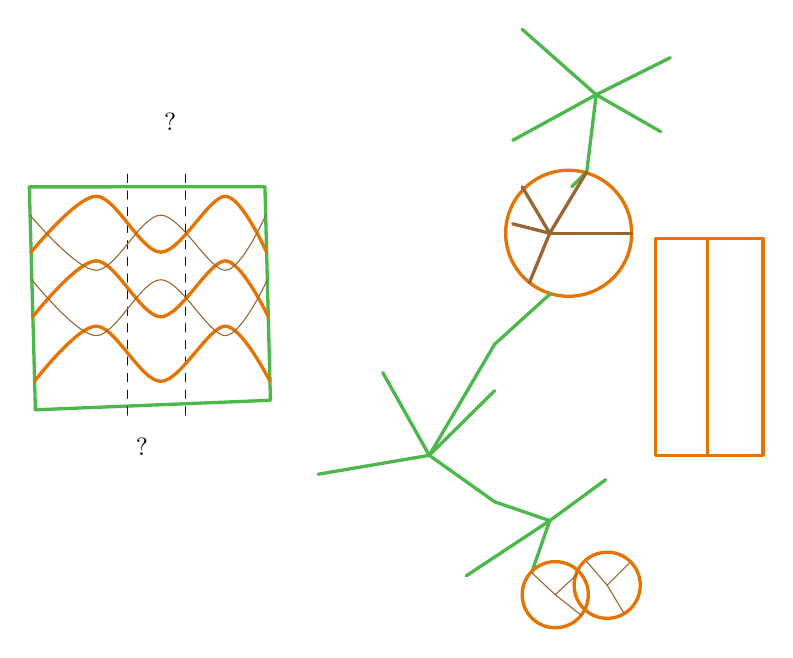
\begin{tikzpicture}[x=1mm,y=1mm,line cap=round,line join=round,font=\scriptsize]
\draw[Lg,very thick] (3.31,-23.51) -- (33.23,-23.49) -- (33.93,-50.61) -- (4.08,-51.82) -- cycle;
\draw[Bl,dashed] (15.8,-21.9) -- (15.8,-52.9);
\draw[Bl,dashed] (23.1,-21.9) -- (23.1,-52.9);
\draw[Or,very thick] plot[smooth, tension=0.55] coordinates {(3.54,-31.8) (11.8,-24.7) (20,-31.8) (28.2,-24.7) (33.45,-31.81)};
\draw[Or,very thick] plot[smooth, tension=0.55] coordinates {(3.76,-39.99) (11.8,-32.9) (20,-40) (28.2,-32.9) (33.66,-40)};
\draw[Or,very thick] plot[smooth, tension=0.55] coordinates {(3.98,-48.18) (11.8,-41.2) (20,-48.2) (28.2,-41.2) (33.87,-48.19)};
\draw[Br] plot[smooth, tension=0.55] coordinates {(3.41,-27.1) (11.8,-34.1) (20,-27.1) (28.2,-34.1) (33.33,-27.11)};
\draw[Br] plot[smooth, tension=0.55] coordinates {(3.63,-35.3) (11.8,-42.4) (20,-35.3) (28.2,-42.4) (33.54,-35.3)};
\node[inner sep=1pt] at (21.2,-15.3) {\small ?};
\node[inner sep=1pt] at (17.6,-56.5) {\small ?};
\draw[Lg,very thick] (75.3,-11.8) -- (65.9,-3.5);
\draw[Lg,very thick] (75.3,-11.8) -- (84.7,-7.1);
\draw[Lg,very thick] (75.3,-11.8) -- (83.5,-16.5);
\draw[Lg,very thick] (75.3,-11.8) -- (64.7,-17.6);
\draw[Lg,very thick] (75.3,-11.8) -- (74.1,-21.6);
\draw[Lg,very thick] (74.1,-21.6) -- (72.2,-23.5);
\draw[Or,very thick] (71.8,-29.4) circle[radius=8];
\draw[Br,very thick] (69.4,-29.4) -- (65.9,-23.5);
\draw[Br,very thick] (69.4,-29.4) -- (74.1,-21.6);
\draw[Br,very thick] (69.4,-29.4) -- (79.8,-29.4);
\draw[Br,very thick] (69.4,-29.4) -- (66.82,-35.66);
\draw[Br,very thick] (69.4,-29.4) -- (64.7,-28.2);
\draw[Lg,very thick] (69.5,-37.06) -- (62.4,-43.5) -- (54.1,-57.6);
\draw[Lg,very thick] (54.1,-57.6) -- (40,-60);
\draw[Lg,very thick] (54.1,-57.6) -- (48.2,-47.1);
\draw[Lg,very thick] (54.1,-57.6) -- (62.4,-49.4);
\draw[Lg,very thick] (54.1,-57.6) -- (62.4,-63.5);
\draw[Lg,very thick] (62.4,-63.5) -- (69.4,-65.9);
\draw[Lg,very thick] (69.4,-65.9) -- (76.5,-60.7);
\draw[Lg,very thick] (69.4,-65.9) -- (58.8,-72.9);
\draw[Lg,very thick] (69.4,-65.9) -- (67.1,-72.5);
\draw[Or,very thick] (70.1,-75.3) circle[radius=4.2];
\draw[Or,very thick] (76.7,-74.1) circle[radius=4.2];
\draw[Br] (70.1,-75.3) -- (67.1,-72.5);
\draw[Br] (70.1,-75.3) -- (72.9,-72.7);
\draw[Br] (70.1,-75.3) -- (73.4,-77.9);
\draw[Br] (76.7,-74.1) -- (74.1,-71.1);
\draw[Br] (76.7,-74.1) -- (79.5,-71.3);
\draw[Br] (76.7,-74.1) -- (78.8,-77.6);
\draw[Or,very thick] (82.8,-30.1) -- (96.5,-30.1) -- (96.5,-57.6) -- (82.8,-57.6) -- cycle;
\draw[Or,very thick] (89.4,-30.1) -- (89.4,-57.6);
\end{tikzpicture}
\end{document}
